\usetikzlibrary{arrows.meta}
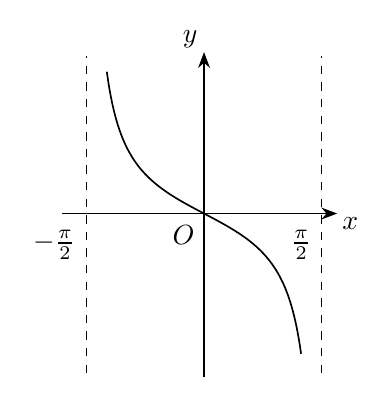
\begin{tikzpicture}[x=0.95cm,y=0.5cm,line width=.6pt,>=Stealth,font=\normalsize]
  \draw[->] (-1.9,0)--(1.78,0);
  \node[anchor=north west,inner sep=1pt] at (1.8,-0.02) {$x$};
  \draw[->] (0,-4.15)--(0,4.1);
  \node[anchor=south east,inner sep=1pt] at (-0.04,4.12) {$y$};
  \draw[dashed] (-1.5708,-4.05)--(-1.5708,4.0);
  \draw[dashed] (1.5708,-4.05)--(1.5708,4.0);
  \draw[domain=-1.30:1.30,samples=201,smooth] plot (\x,{-tan(deg(\x))});
  \node[anchor=north east,inner sep=1.5pt] at (-0.06,-0.18) {$O$};
  \node[anchor=east,inner sep=2pt] at (-1.64,-0.80) {$-\frac{\pi}{2}$};
  \node[anchor=east,inner sep=2pt] at (1.52,-0.80) {$\frac{\pi}{2}$};
\end{tikzpicture}
